\section{1st Model}
\label{sec:Model}

In an effort to create a working trust model iteratively, we will start by simplifying the model described by Castelfranchi and Falcone \cite{Castelfranchi1998}, by removing the effects of outside influence in Trust. We also do not take into account long term considerations of the trustor's goal, reducing contextual scope to just the task being performed by the trustor. So Trust is represented by a 3-tuple:

\begin{itemize}
	\item The trustor (\textbf{X});
	\item The trustee (\textbf{Y});
	\item A task ($\bm{\tau}$) defined by the pair $(\alpha, \rho)$, where \bm{$\alpha$} is the action entrusted to the trustee, that possibly produces an outcome \bm{$\rho$}, contained in the goal of \textbf{X}.
\end{itemize}
\begin{equation}
TRUST(X\ Y\ \tau)
\label{eq:TrustRelation}
\end{equation}

We seek to represent the trustee as a set of features from which an overall evaluation may be retrieved. These features provide a representation of the trustee's abilities in various fields, as well as concerns related to willingness, such as task preference. So a trustee $Y$'s feature set $ S_y $ can be as seen in \ref{eq:FeaturesExample}.
\begin{equation}
S_y=\left\{cooking, writing, preference\ to\ cook\right\}
\label{eq:FeaturesExample}
\end{equation}
These features must be able to provide 2 values:

\begin{itemize}
	\item trust - a value for how much trust we have in this trustee's specific feature;
	\item certainty - the degree of how much we believe this trust assumption to be true, tanking into account factors like how many times, or how long ago did we last affirm this belief.
\end{itemize}

This makes it easier to visualize a certain trustee's trust reasoning, as we can observe all the factors that contribute towards an evaluation. The specificity of the concrete features is purposefully left generic in order make the model fit in different scenarios. This makes the model dependent on an ontology specific for the scenario, but we think this concern is unavoidable if we want to have understandable models, as the alternative solution is to use machine learning to perform clustering, which are difficult to describe most of the time. 


Trust and certainty are calculated through a collection of belief sources, which in the first version will be a history of direct contacts. The environment must be able to provide some way to access these contacts, either by a callback function or through open access to an action history. If the environment does not provide such features, a perception module, capable of checking action results, will be required.

The task is composed by a set of related features with a given weight. This represents the features most closely related to the task at hand, and their importance to he completion of the task.


\begin{figure}[hbt]
	\centering
	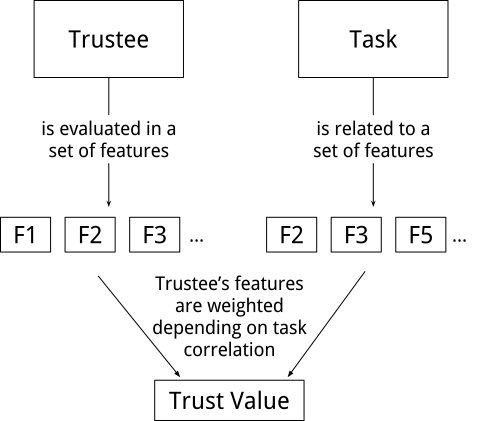
\includegraphics[height=200px]{figures/Trust_Model_Diagram.png}
	\caption{Trustee Features Representation}
	\label{fig:trustee}
\end{figure}


\subsection{Implementation}

Implementation wise, the model will be first implemented by using a simple class structure, as seen in figure \ref{fig:classDiagram}. In this diagram, the main actor is the Agent, which contains a list of Trustees with features that the Agent has been able to perceive from received sources. For now the sources must be given by the simulation environment, but an interpreter should be implemented to sort out and transform the perceptions received by the environment into sources for belief features.
A simple simulation example can be performed as following:
\begin{enumerate}
	\item Instantiate Agent A(nna) and Agent B(ob);
	\item Instantiate Trustee B and assign as A's trustee;
	\item Insert Direct Contact Source with Feature ID "Cooking"; this should create a new Trust Feature in Trustee B;
	\item Calculate Trust with task "Cook";
\end{enumerate}

\begin{figure}[hbt]
	\centering
	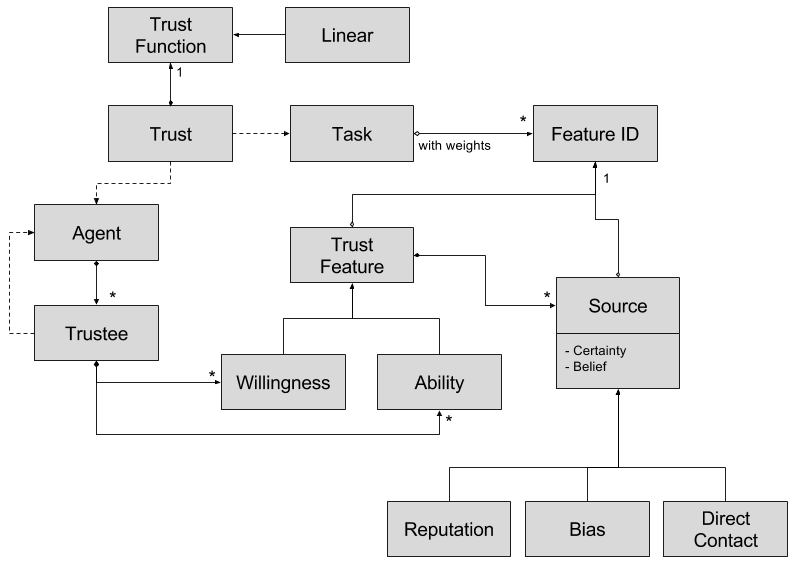
\includegraphics[height=250px]{figures/Class_Diagram.png}
	\caption{Class Diagram}
	\label{fig:classDiagram}
\end{figure}

\section{Example Case}



